%=== Einheit Codierungen =====================================================
\Tut\chapter{\"Ubersetzungen und Codierungen}
\label{k:codierungen}

Von natürlichen Sprachen weiß man, dass man \emph{übersetzen}
kann. Beschränken wir uns im weiteren der Einfachheit halber als
erstes auf Inschriften. Was ist dann eine Übersetzung? Das hat zwei
Aspekte:
\begin{enumerate}
\item eine Zuordnung von Wörtern einer Sprache zu Wörtern einer
  anderen Sprache, die
\item die schöne Eigenschaft hat, dass jedes Ausgangswort und
  seine Übersetzung die gleiche Bedeutung haben.
\end{enumerate}
%
Als erstes schauen wir uns ein einfaches Beispiel für Wörter und ihre
Bedeutung an: verschiedene Methoden der Darstellung natürlicher
Zahlen.

%-----------------------------------------------------------------------
\Tut\section{Von W\"ortern zu Zahlen und zur\"uck}

%-----------------------------------------------------------------------
\Tut\subsection{Dezimaldarstellung von Zahlen}

Wir sind gewohnt, natürliche Zahlen im sogenannten Dezimalsystem
notieren, das aus Indien kommt (siehe auch
Kapitel~\ref{k:algorithmusbegriff} über den Algorithmusbegriff):
%
\begin{itemize}
\item Verwendet werden die Ziffern des Alphabetes
  $Z_{10}=\{\literal{0}, \dots, \literal{9}\}$. 
\item Die Bedeutung $\fnum_{10}(x)$ einer einzelnen Ziffer $x$ als
  Zahl ist durch die folgende Tabelle gegeben:

  {
    \setlength{\abovetopsep}{1ex}
    \setlength{\belowbottomsep}{1ex}
    \qquad
    \begin{tabular}{c@{\quad}*{10}{>{$}c<{$}}}
      \toprule
      $x$ & \literal{0}&\literal{1}&\literal{2}&\literal{3}&\literal{4}
      &\literal{5}&\literal{6}&\literal{7}&\literal{8}&\literal{9}\\
      $\fnum_{10}(x)$ & 0&1&2&3&4&5&6&7&8&9\\ %
      \bottomrule
    \end{tabular}
  }

  \noindent
  Man beachte, dass in der ersten Zeile der Tabelle \emph{Zeichen}
  stehen, und in der zweiten Zeile \emph{Zahlen}. Genauer gesagt
  stehen in der ersten Zeile Zeichen, die für sich stehen, und in der
  zweiten Zeile Zeichen, die Sie als Zahlen interpretieren sollen.
  
  Also ist $\fnum_{10}$ eine Abbildung $\fnum_{10}\colon Z_{10} \to \G_{10}$.

\item Für die Bedeutung eines ganzen Wortes $x_{k-1} \cdots x_0\in
  Z_{10}^*$ von Ziffern wollen wir $\fNum_{10}(x_{k-1} \cdots x_0)$
  schreiben. In der Schule hat man gelernt, dass das gleich
  \[
  10^{k-1}\cdot \fnum_{10}(x_{k-1}) + \cdots + 10^1\cdot \fnum_{10}(x_1)
  + 10^0\cdot \fnum_{10}(x_0)
  \]
  ist. Wir wissen inzwischen, wie man die Pünktchen vermeidet. Und da
  \begin{multline*}
    10^{k-1}\cdot \fnum_{10}(x_{k-1}) + \cdots + 10^1\cdot \fnum_{10}(x_1)
    + 10^0\cdot \fnum_{10}(x_0) \\
    = 10\left(10^{k-2}\cdot \fnum_{10}(x_{k-1}) + \cdots + 10^0\cdot \fnum_{10}(x_1)\right)
    + 10^0\cdot \fnum_{10}(x_0)
  \end{multline*}
  ist, definiert man $\fNum_{10}\colon Z_{10}^* \to\N_0$ so:
  %
  \begin{align*}
    \fNum_{10}(\eps) &= 0  \\ %\label{eq:foo1}
    \text{für jedes }  w\in Z_{10}^* \,\, \text{für jedes }  x\in Z_{10}: \fNum_{10}(wx) &= 10\cdot \fNum_{10}(w) + \fnum_{10}(x) \\ %\label{eq:foo2}
  \end{align*}
\end{itemize}
%
\begin{tutorium}
\noindent\textbf{$\fNum_{10}$}
  \begin{align}
    \fNum_{10}(\eps) &= 0  \label{eq:foo1} \\
    \text{für jedes }  w\in Z_{10}^* \,\, \text{für jedes }  x\in Z_{10}: \fNum_{10}(wx) &= 10\cdot \fNum_{10}(w) + \fnum_{10}(x) \label{eq:foo2} 
  \end{align}


  \begin{itemize}
  \item noch ein Beispiel oder langweilig?
  \item Beweis, dass Definition sinnvoll:

    \begin{lemma}
      Durch die Gleichungen~\ref{eq:foo1} und~\ref{eq:foo2} ist
      $\fNum_{10}$ wohldefiniert, das heißt, für jedes Wort $w\in Z^*$
      wird eindeutig der Funktionswert $\fNum_{10}(w)$ festgelgt.
    \end{lemma}

    Um das mittels vollständiger Induktion zu beweisen, formulieren
    wir etwas um:

    \begin{lemma}
      Durch die Gleichungen~\ref{eq:foo1} und~\ref{eq:foo2} ist
      $\fNum_{10}$ wohldefiniert, das heißt, 

      für jede Wortlänge $n\in\N_0$ gilt: für alle $w\in Z^n$
      wird eindeutig der Funktionswert $\fNum_{10}(w)$ festgelgt.
    \end{lemma}

    \begin{beweis}
      Beweis durch Induktion über die Wortlänge $n$:

      \begin{description}
      \item[Induktionsanfang $n=0$:] In diesem Fall ist zu beweisen: Für
        jedes Wort $w$ der Länge $n=0$ ist $\fNum_{10}(w)$ festgelegt, und
        zwar eindeutig.

        Das ist leicht: Wenn $|w|=0$ ist, dann ist $w=\eps$. Tatsächlich
        legt Gleichung~(\ref{eq:foo1}) offensichtlich eindeutig einen
        Funktionswert $\fNum_{10}(\eps)$ fest, nämlich $0$. Und
        Gleichung~(\ref{eq:foo2}) legt \emph{keinen} Funktionswert für
        $\fNum_{10}(\eps)$ fest, denn die auf der linken Seite
        auftretenden Argumente haben alle eine Länge
        $|wx|=|w|+|x|=|w|+1\geq 1$, sind also ganz bestimmt \emph{nicht}
        das leere Wort.
      \item[Induktionsvoraussetzung:] für ein beliebiges aber festes
        $n\in\N_0$ gelte: Für alle Wörter $w\in Z^n$ ist
        $\fNum_{10}(w)$ eindeutig definiert.
      \item[Induktionsschritt $n\leadsto n+1$:] Nun müssen wir beweisen, dass die
        Richtigkeit der Aussage des Lemmas für ein $n$ zwingend auch die
        Richtigkeit der Aussage für $n+1$ nach sich zieht.
        
        Bezeichne $w'$ ein beliebiges Wort der Länge $n+1$. Wir müssen
        zeigen: $\fNum_{10}(w')$ ist eindeutig festgelegt. Das geht
        so:

        Wenn $|w'|=n+1$, dann enthält $w'$ mindestens ein Symbol, also
        auch ein letztes. Bezeichnen wir das mit $x$. Dann ist $w'$ von
        der Form $w'=wx$ mit $w\in Z^n$ und $x\in Z$.

        In der Definition von $\fNum_{10}$ passt \emph{nur} Gleichung~\ref{eq:foo2}:
        \[
        \fNum_{10}(w')=\fNum_{10}(wx) = 10\cdot \fNum_{10}(w) + \fnum_{10}(x)
        \]
        Nach IV ist $\fNum_{10}(w)$ eindeutig festgelegt, also auch
        $\fNum_{10}(w')$.
    \end{description}
    \end{beweis}
  \end{itemize}
\end{tutorium}


%-----------------------------------------------------------------------

\Tut\subsection{Andere unbeschr\"ankte Zahldarstellungen}

\begin{window}[0,r,\includegraphics[width=28mm]{../k-08-codierungen/Leibniz},{Gottfried Wilhelm Leibniz}]
\noindent\personname{Gottfried Wilhelm Leibniz} wurde am 1.~Juli 1646 in Leipzig geboren
und starb am 14.~November 1716 in Hannover. Er war Philosoph,
Mathematiker, Physiker, Bibliothekar und vieles mehr.  Leibniz baute
zum Beispiel die erste Maschine, die zwei Zahlen multiplizieren
konnte.

Leibniz hatte erkannt, dass man die natürlichen Zahlen nicht nur mit
den Ziffern $\literal{0}, \dots, \literal{9}$ notieren kann, sondern
dass dafür $\literal{0}$ und $\literal{1}$ genügen. Er hat dies in
einem Brief vom 2.~Januar 1697 an den Herzog von
Braunschweig-Wolfenbüttel beschrieben
\end{window}
(siehe auch
\url{http://www.hs-augsburg.de/~harsch/germanica/Chronologie/17Jh/Leibniz/lei_bina.html},
10.11.2015) und im Jahre 1703 in einer Zeitschrift veröffentlicht.
Abbildung~\ref{abb:leibniz-binaer} zeigt Beispielrechnungen mit Zahlen
in Binärdarstellung aus dieser Veröffentlichung.

\begin{figure}[ht]
  \centering
  \includegraphics[scale=2.5,bb=47 67 160 156,clip]{../k-08-codierungen/Leibniz_binary_system_1703}
  \caption{Ausschnitt aus dem Aufsatz "`Explication de l'Arithmétique
    Binaire"' von Leibniz, Quelle:
    \url{http://commons.wikimedia.org/wiki/Image:Leibniz_binary_system_1703.png}
    (10.11.2015)}
  \label{abb:leibniz-binaer}
\end{figure}

\noindent
Bei der \mdefine{Binärdarstellung}\index{Binärdarstellung} von
nichtnegativen ganzen Zahlen geht man analog zur Dezimaldarstellung
vor. Als Ziffernmenge benutzt man $Z_2=\{\literal{0}, \literal{1}\}$
und definiert
\begin{align*}
   \fnum_2(\literal{0}) &= 0 \\
   \fnum_2(\literal{1}) &= 1 \\
   \fNum_2(\eps) &= 0 \\
\text{sowie \qquad }\text{für jedes }  w\in Z_2^* \,\, \text{für jedes }  x\in Z_2:  \fNum_2(wx) &= 2\cdot \fNum_2(w) +\fnum_2(x)
\end{align*}
%
Damit ist dann \zB 
%
\begin{align*}
  \fNum_2(\literal{1101}) &= 2\cdot  \fNum_2(\literal{110}) +1 \\
  &= 2\cdot (2\cdot  \fNum_2(\literal{11}) + 0) +1 \\
  & = 2 \cdot(2\cdot (2\cdot\fNum_2(\literal{1})+ 1)+0 ) +1 \\
  & = 2 \cdot(2\cdot (2\cdot1+ 1)+0 ) +1 \\
  & = 2^3\cdot 1 + 2^2 \cdot 1 + 2^1 \cdot 0 + 2^0 \cdot 1 \\
  & = 13
\end{align*}
%
\begin{tutorium}
  \noindent\textbf{Beispielrechungen}
  \begin{itemize}
  \item klar machen, wie allgemein bei Basis $k$ die Umwandlung
    funktioniert: $\fNum_k(wx) = k\cdot \fNum_k(w) +\fnum_k(x)$.
  \item Beispiel rechnen, z.B. $\fNum_3(\#{111})= \dots = 13$.
  \item $\fNum_2(\#{1})=1$, $\fNum_2(\#{11})=3$, $\fNum_2(\#{111})=7$,
    $\fNum_2(\#{1111})=15$,

    Wer sieht allgemein: $\text{für jedes }  m\in \N_0: \fNum_2(\literal{1}^m) = 2^m-1$?

    Wie überträgt sich das auf den Fall $k=3$? $\text{für jedes }  m\in \N_0:
    \fNum_3(\literal{2}^m) = 3^m-1$.
  % \item Und dann vielleicht noch die folgende Spielerei:
  %   \begin{itemize}
  %   \item $Z'_3=\{\literal{1}, \literal{0},
  %     \literal{\meins}\}$ mit \\
  %     $\fnum'_3(\literal{\meins}) = -1$, $\fnum'_3(\literal{0}) = 0$,
  %     und $\fnum'_3(\literal{1}) = 1$ sowie
  %     \begin{align*}
  %       \fNum'_3(\eps) &= 0 \\
  %       \text{für jedes }  w\in {Z'_3}^* \,\, \text{für jedes }  x\in Z'_3:
  %       \fNum'_3(wx) &= 3\cdot \fNum'_3(w) +\fnum'_3(x)
  %     \end{align*}
  %   \item Man berechne erst mal \zB $\fNum'_3(\literal{\meins10})$
  %     (gibt $-6$) und $\fNum'_3(\literal{1\meins1})$ (gibt $7$)
  %   \item Was passiert, wenn man in einer Zahldarstellung aus allen
  %     $\#1$ ein $\#{\meins}$ macht und umgekehrt?: Darstellung der
  %     entsprechenden negierten Zahl.
      
  %     Z.B. $\fNum'_3(\literal{\meins1\meins}) = - \fNum'_3(\literal{1\meins1}) = 6$
  %   \end{itemize}
  \end{itemize}
\end{tutorium}

% \begin{tutorium}
%   \noindent\textbf{Algorithmus für Umwandlung von Binärdarstellung nach Zahl erarbeiten:}
%   \begin{align*}
%     & \assert{\text{Eingabe: } w\in Z_2^*} \\
%     & x <- 0 \\
%     &\kw{for\ } i<-0 \kw{\ to\ } |w| -1 \kw{ do}\\
%     & \qquad x <- 2x + \fnum_2(w(i)) \\
%     &\kw{od} \\
%     & \assert{\text{am Ende: } x=\fNum_2(w)} 
%   \end{align*}
%   Die Schleifeninvariante sieht man besser bei
%   \begin{align*}
%     & \assert{\text{Eingabe: } w\in Z_2^*} \\
%     & x <- 0 \\
%     & v <- \eps \\
%     &\kw{for\ } i<-0 \kw{\ to\ } |w| -1 \kw{ do}\\
%     & \qquad v <- v \cdot w(i)\\
%     & \qquad x <- 2x + \fnum_2(w(i)) \\
%     &\kw{od} \\
%     & \assert{\text{am Ende: } v=w \land x=\fNum_2(w)} 
%   \end{align*}
%   % 
%   Suchen lassen: $x=\fNum_2(v)$

%   Dass das eine Schleifeninvariante ist, nicht in allen Details
%   beweisen.  Aber den Kern erkennen: laut Definition von $\fNum_2$ ist
%   nämlich
%   \[
%   \fNum_2(v\cdot w(i)) = 2 \fNum_2(v) + \fnum_2(w(i))
%   \]
% \end{tutorium}
%
Bei der \mdefine{Hexadezimaldarstellung}\index{Hexadezimal-\\darstellung}
oder Sedezimaldarstellung benutzt man $16$ Ziffern des Alphabets
$Z_{16}=\{\literal{0}$, $\literal{1}$, $\literal{2}$, $\literal{3}$,
$\literal{4}$, $\literal{5}$, $\literal{6}$, $\literal{7}$,
$\literal{8}$, $\literal{9}$, $\literal{A}$, $\literal{B}$,
$\literal{C}$, $\literal{D}$, $\literal{E}$,
$\literal{F}\}$. (Manchmal werden statt der Großbuchstaben auch
Kleinbuchstaben verwendet.)

\begin{center}
   \begin{tabular}{c@{\qquad}*{16}{>{$}c<{$}}}
    \toprule
    $x$ & \literal{0}&\literal{1}&\literal{2}&\literal{3}&\literal{4}&\literal{5}&\literal{6}&\literal{7} \\
    $\fnum_{16}(x)$ & 0&1&2&3&4&5&6&7\\ %
    \midrule
    $x$ & \literal{8}&\literal{9}&\literal{A}&\literal{B}&\literal{C}&\literal{D}&\literal{E}&\literal{F}\\
    $\fnum_{16}(x)$ & 8&9&10&11&12&13&14&15\\ %
    \bottomrule
  \end{tabular}
\end{center}
%
Die Zuordnung von Wörtern zu Zahlen ist im Wesentlichen gegeben durch
\[
\text{für jedes }  w\in Z_{16}^* \,\, \text{für jedes }  x\in Z_{16}: \fNum_{16}(wx) =
16\cdot \fNum_{16}(w) +\fnum_{16}(x)
\]
%
Ein Problem ergibt sich dadurch, dass die Alphabete $Z_2$, $Z_3$, \usw
nicht disjunkt sind. Daher ist \zB die Zeichenfolge $\literal{111}$
mehrdeutig: Um sagen zu können, welche Zahl hier repräsentiert wird,
muss man wissen, zu welcher Basis die Zahl dargestellt ist.  Zum
Beispiel ist
%
\begin{center}
  \begin{tabular}{ll}
    $\fNum_2(\literal{111})$  & die Zahl sieben, \\
    $\fNum_8(\literal{111})$  &  die Zahl dreiundsiebzig, \\
    $\fNum_{10}(\literal{111})$ &  die Zahl einhundertelf und \\
    $\fNum_{16}(\literal{111})$ & die Zahl zweihundertdreiundsiebzig.
  \end{tabular}
\end{center}
% 
Deswegen ist es in manchen Programmiersprachen so, dass für
Zahldarstellungen zu den Basen $2$, $8$ und $16$ als Präfix respektive
$\literal{0b}$, $\literal{0o}$ und $\literal{0x}$ vorgeschrieben
sind. Dann sieht man der Darstellung unmittelbar an, wie sie zu
interpretieren ist. In anderen Programmiersprachen sind entsprechende
Darstellungen gar nicht möglich.


%-----------------------------------------------------------------------
\Tut\subsection{Ganzzahlige Division mit Rest}

So wie man zu einem Wort die dadurch repräsentierte Zahl berechnen
kann, kann man auch umgekehrt zu einer nichtnegativen ganzen Zahl
$n\in\N_0$ eine sogenannte $k$-äre Darstellung berechnen. 

Um das einzusehen betrachten wir als Vorbereitung zwei binäre
Operationen, die Ihnen im Laufe dieser und anderer Vorlesungen noch
öfter über den Weg laufen werden.
%
Sie heißen \mdefine{\emph{\kw{div}}}\index{div} und
\mdefine{\emph{\kw{mod}}}\index{mod} und sind wie folgt definiert: 
%
Die Operation $\kw{mod}$
liefert für zwei Argumente $x\in\N_0$
und $y\in\N_+$
als Funktionswert $x\kw{\ mod\ }y$
den Rest der ganzzahligen Division von $x$
durch $y$.
%
Und die Operation $\kw{div}$
liefere für $x\in\N_0$
und $y\in\N_+$
als Funktionswert $x\kw{\ div\ }y$
den Wert der ganzzahligen Division von $x$
durch $y$. 
%
Mit anderen Worten gilt stets:
\begin{equation}
  x = y\cdot (x\kw{\ div\ }y) + (x\kw{\ mod\ }y)  
  \text{\qquad und \qquad} 0 \leq (x\kw{\ mod\ }y) < y\label{eq:div-mod}
\end{equation}
%
\begin{tutorium}
  \noindent\textbf{Rechnen mit div und mod}
  \begin{equation*}
    x = y\cdot (x\kw{\ div\ }y) + (x\kw{\ mod\ }y)  
    \text{\qquad und \qquad} 0 \leq (x\kw{\ mod\ }y) < y
  \end{equation*}
  \begin{itemize}
  \item Bitte das Rechnen mit \kw{\ div\ } und \kw{\ mod\ } üben.
    
    Vielleicht mal einfach eine Tabelle ausfüllen (lassen) der Form

    \begin{tabular}{>{$}l<{$}|*{12}{>{$}c<{$}}}
      x & 0 & 1 & 2 & 3 & 4 & 5 & 6 & 7 & 8 & 9 & 10 & 11 \\
      x\kw{\ div\ } 4 & 0& 0& 0& 0&1&1&1&1&2&2 &2&2\\
      4(x\kw{\ div\ } 4) & 0& 0& 0& 0&4&4&4&4&8&8&8&8 \\
      x\kw{\ mod\ } 4 & 0&1&2&3& 0&1&2&3&0&1&2&3\\
    \end{tabular}
  \item Klar machen, dass $x\kw{\ mod\ }2$ was mit gerade und ungerade
    zu tun hat.
  \end{itemize}
\end{tutorium}
%
Etwas anders ausgedrückt gilt das folgende:
%
Wenn eine Zahl $x\in\N_0$
für ein $k\in\N_+$
in der Form $x=k\cdot p_x + r_x$
dargestellt ist, wobei $p_x\in\N_0$
und $0\leq r_x<k$, also $r_x\in\G_k$,
ist, dann ist gerade $p_x=x\kw{ div }k$ und $r_x=x\kw{ mod }k$.

Hieraus ergibt sich schnell folgendes Lemma.

\begin{lemma}
  Für jede $x,y\in\N_0$ und jedes $k\in\N_+$ gilt:
  \[
    (x+y)\kw{ mod }k = ((x \kw{ mod }k) + (y\kw{ mod }k)) \kw{ mod }k
  \]
\end{lemma}

\begin{beweis}
  Es sei $x=k\cdot p_x + r_x$
  und $y=k\cdot p_y + r_y$ mit $r_x,r_y\in\G_k$. Dann ist 
  \begin{align*}
    (x+y)\kw{ mod }k &= (k p_x + r_x + kp_y + r_y)\kw{ mod }k\\
                     &= (r_x + r_y)\kw{ mod }k \\
                     &= ((x \kw{ mod }k) + (y\kw{ mod }k)) \kw{ mod }k
  \end{align*}
\end{beweis}


%-----------------------------------------------------------------------
\Tut\subsection{Von Zahlen zu ihren Darstellungen}

Es sei nun $k\geq 2$.

Mit Hilfe der beiden eben eingeführten Funktionen kann man dann eine
sogenannte \mdefine{$k$-äre
  Darstellung}\index{Darstellung von Zahlen} oder auch
\mdefine{$k$-äre
  Repräsentation}\index{Repräsentation von Zahlen} einer Zahl
festlegen.
%
Dazu benutzt man ein Alphabet $Z_k$
mit $k$ Ziffern, deren Bedeutungen die Zahlen in $\G_k$ sind.
%
Für $i\in\G_k$ sei $\frepr_k(i)$ dieses Zeichen.
%
Die Abbildung $\frepr_k$
ist also gerade die Umkehrfunktion zu $\fnum_k$.

Gesucht ist nun eine Repräsentation von $n\in\N_0$ als Wort $w\in
Z^*_k$ mit der Eigenschaft $\fNum_k(w)=n$. Dabei nimmt man die
naheliegende Definition von $\fNum_k$ an.

Wie wir gleich sehen werden, gibt es immer solche Wörter. Und es sind
dann auch immer gleich unendlich viele, denn wenn $\fNum_k(w)=n$ ist,
dann auch $\fNum_k(\literal{0}w)=n$ (einfach nachrechnen). 

Die Funktion $\fRepr_k$ definieren wir so:
%
\begin{samepage}
\begin{align}
  \fRepr_k(n) =
  \begin{cases}
    \frepr_k(n) & \text{ falls } n < k \\
    \fRepr_k(n \kw{ div } k) \cdot \frepr_k(n \kw{ mod } k) & \text{ falls } n \geq k
  \end{cases}
                                                              \label{l:def-Repr}
\end{align}
%
Dabei bedeutet der Punkt $\cdot$ in der zweiten Zeile Konkatenation.
\end{samepage}
%
Hier liegt wieder einmal ein induktive Definition vor, aber es ist
nicht so klar wie bisher, dass tatsächlich für jedes $n\in\N_0$
ein Funktionswert $\fRepr_k(n)$ definiert wird.
%
Daher wollen wir das beweisen.
%
Genauer betrachten wir für $m\in\N_+$ die Aussagen $\A_m$ der Form:
\begin{quote}
  "`Für alle $n\in\N_n$ mit $n< k^m$ ist $\fRepr_k(n)$ definiert."'
\end{quote}
oder anders aber äquivalent formuliert:
\begin{quote}
  "`Für alle $n\in\N_n$
  gilt: Wenn $n< k^m$ ist, dann ist $\fRepr_k(n)$ definiert."'
\end{quote}
%
Im \emph{Induktionsanfang} müssen wir Aussage $\A_1$
beweisen, die besagt, dass $\fRepr_k(n)$
für alle $n\in\N_0$ mit $n<k$ definiert ist.
%
Das ist aber klar, denn dann ist laut~(\ref{l:def-Repr}) gerade
$\fRepr_k(n)=\frepr_k(n)$.

Für den Induktionsschritt sei nun $m\in\N_+$.
%
Als \emph{Induktionsvoraussetzung} können wir benutzen:
\begin{quote}
  "`Für alle $n\in\N_n$ mit $n< k^m$ ist $\fRepr_k(n)$ definiert."'
\end{quote}
%
Zu zeigen ist, dass dann auch gilt:
\begin{quote}
  "`Für alle $n\in\N_n$ mit $n< k^{m+1}$ ist $\fRepr_k(n)$ definiert."'
\end{quote}
%
Sei also $n\in\N_0$ und $n< k^{m+1}$.
%
Dann sind zwei Fälle möglich:
\begin{itemize}
\item Es ist sogar $n< k^m$.
  %
  Dann ist $\fRepr_k(n)$ gemäß der Induktionsvoraussetzung definiert.
\item Es ist $k^m\leq n< k^{m+1}$.
  %
  Dann ist $n\kw{ div }k< k^m$
  und somit nach Induktionsvoraussetzung $\fRepr_k(n\kw{ div }k)$
  definiert.
  %
  Folgich ist aber wieder nach~(\ref{l:def-Repr}) auch
  $\fRepr_k(n) =\fRepr_k(n \kw{ div } k) \cdot \frepr_k(n \kw{ mod }
  k)$ definiert.
\end{itemize}
% 
% \Begin{align*}
%   &\assert{\text{Eingabe: } n\in\N_0} \\
%   &y <- n \\
%   &w <- \eps \\
%   &m <- \begin{cases}
%     1 + \lfloor\log_k(n)\rfloor & \text{ falls } n>0 \\
%     1 & \text{ falls } n=0
%     \end{cases}\\
%   &\kw{for\ } i<-0 \kw{\ to\ } m-1 \kw{ do}\\
%   & \qquad r <- y \kw{\ mod\ } k \\
%   & \qquad w <- \frepr_k(r)\cdot w \text{\qquad // Konkatenation}\\
%   & \qquad y <- y \kw{\ div\ } k  \\ 
%   &\kw{od} \\
%   & \assert{\text{am Ende: } n=\fNum_k(w)}  
% \end{align*} 
%
% Am deutlichsten wird die Arbeitsweise dieses Algorithmus, wenn man ihn
% einmal für einen vertrauten Fall benutzt: Nehmen wir $k=10$ und
% $n=4711$. Dann ist $m=4$ und für jedes $i\in\G_5$ haben die Variablen
% $r$, $w$ und $y$ nach $i$ Schleifendurchläufen die in der folgende
% Tabelle angegebenen Werte. Um die Darstellung besonders klar zu
% machen, haben wir die Fälle von $i=0$ bis $i=4$ von rechts nach links
% aufgeschrieben:
% %
% \begin{center}
%   \setlength{\abovetopsep}{1ex}
%   \setlength{\belowbottomsep}{1ex}
%   \begin{tabular}{*{6}{>{$}c<{$}}}
%     \toprule
%     i & 4 & 3 & 2 & 1 & 0 \\
%     \midrule
%     r & 4 & 7 & 1 & 1 &   \\
%     w & \#{4711} & \#{711} & \#{11} & \#{1} & \eps \\
%     y & 0 & 4 & 47 & 471 & 4711 \\
%     \bottomrule
%   \end{tabular}
% \end{center}
% %
% Die Schleifeninvariante $y \cdot 10^i + \fNum_{k}(w) = n$ drängt sich
% förmlich auf. Und wenn man bewiesen hat, dass am Ende $y=0$ ist, ist
% man fertig.
%
% \begin{tutorium}
%   Eventuell noch mal die Spielerei mit $\fNum'_3$:
%   \begin{itemize}
%   \item Welche positiven Zahlen haben eine Repräsentation? Welche
%     negativen?  (Antwort: alle alle) Und die Null geht natürlich auch.
%   \item Hinweis: Im Rechner benutzt man aber nur
%     $\Z_2=\{\#0,\#1\}$. Da muss man sich was anderes überlegen für
%     negative Zahlen.
%   \item sieht man ähnlich wie oben, Modifikation erarbeiten
%   \end{itemize}
% \end{tutorium}

Es sei noch angemerkt, dass mit Ausnahme der $0$
die Funktion $\fRepr_k$
zu gegebenem $n\in\N_0$
das (es ist eindeutig) kürzeste Wort $w\in Z_k^*$ mit $\fNum_k(w)=n$.
%
Es ist also stets
\[
\fNum_k(\fRepr_k(n)) = n \;.
\]
Man beachte, dass umgekehrt $\fRepr_k(\fNum_k(w))$ im allgemeinen
nicht unbedingt wieder $w$ ist, weil "`überflüssige"' führende Nullen
wegfallen.

%-----------------------------------------------------------------------
\Tut\subsection{Beschr\"ankte Zahlbereiche und Zahldarstellungen}

In Kapitel~\ref{k:prozessor} werden Sie ein erstes Modell für
Prozessoren kennenlernen, die (mikroprammierte) \emph{Minimalmaschine}
\mima. 
%
Sie ist nicht wirklich minimal, aber an einigen Stellen wird sie im
Vergleich zu realen Prozessoren wie Sie in Desktop"=Rechnern,
Mobiltelefonen und anderen Geräten verbaut sind, stark vereinfacht
sein. 
%
Wichtige Aspekte werden aber auch schon an der \mima sichtbar werden.

Dazu gehört, dass man nicht beliebig große Zahlen repräsentieren kann.
%
Einzelne Zahlen (und auch anders zu interpretierende Objekte) werden
in sogenannten \emph{Registern} gespeichert werden, und zwar in der
\mima immer als Bitwörter der Länge $24$. 
%
In einem Register lassen sich also maximal $2^{24}$
verschiedene Zahlen speichern. 
%
Die Frage ist: welche und in welcher Repräsentation?

Eine einfache (aber nicht zutreffende) Vorgehensweise wäre diese: 
%
\begin{itemize}
\item Für $\ell\in\N_+$ sei die Funktion
  $\fbin_{\ell}\colon \G_{2^{\ell}} \to \{\#0,\#1\}^{\ell}$ definiert
  vermöge der Festlegung
  \[
  \fbin_{\ell}(n) = \#0^{\ell- |\fRepr_2(n)|} \fRepr_2(n)
  \]
  Es ist also stets $|\fbin_{\ell}(n)| =\ell$ und $\fNum_2(\fbin_{\ell}(n))=n$.
\item Dann könnte man in der \mima jede Zahl $n\in \G_{2^{24}}$ in der
  Form $\fbin_{24}(n)$ darstellen.
\end{itemize}
% 
Aber "`natürlich"' möchte man auch negative Zahlen repräsentieren
können. 
%
Und es wäre praktisch, wenn man für deren Verarbeitung keine extra
Recheneinheiten benötigen würde, sondern \zB ein sogenanntes
Addierwerk immer das Gewünschte leistet, gleich, ob die Argumente für
negative oder für nichtnegative Zahlen stehen.

Es zeigt sich, dass man das tatsächlich erreichen kann. 
%
Im Folgenden stellen wir eine solche Repräsentation vor, die
sogenannte
\mdefine{Zweierkomplement"=Darstellung}\index{Zweierkomplement}.

Auch dafür muss man als erstes eine \emph{feste Länge} der
Zahldarstellungen festlegen. 
%
Wir bezeichnen Sie mit $\ell$.
%
Es ist $\ell\in\N_+$ und sinnvollerweise $\ell\geq 2$.
%
Die Menge der Zahlen, die man in Zweierkomplementdarstellung der Länge
$\ell$ repräsentieren kann ist
%
\begin{samepage}
\[
\ZK_{\ell} = \{ x\in \Z \mid -2^{\ell-1} \leq x \leq 2^{\ell-1} -1 \} \;.
\]
%
(Dabei schreiben wir "`$a\leq b\leq c$"'
als Abkürzung für "`$a\leq b$ und $b\leq c$"'.)
\end{samepage}
% 
Es sind also \zB
\begin{align*}
  \ZK_2 &= \{ -2, -1, 0, 1\} \\
   \text{  und   \qquad }  \ZK_8 &= \{ -128, -127, \dots, -1, 0, 1, \dots, 127 \}
\end{align*}
%
Die Zweierkomplementdarstellung
$\fZkpl_{\ell}\colon \ZK_{\ell} \to \{\#0,\#1\}^{\ell}$ der Länge
$\ell$ ist für alle $x\in\ZK_{\ell}$ wie folgt definiert:
\[
\fZkpl_{\ell}(x) =
\begin{cases}
  \#0 \fbin_{\ell-1}(x) & \text{ falls } x\geq 0 \\
  \#1 \fbin_{\ell-1}(2^{\ell-1} + x) & \text{ falls } x< 0 
\end{cases}
\]
%
Man kann sich überlegen, dass auch gilt:
\[
\fZkpl_{\ell}(x) =
\begin{cases}
  \fbin_{\ell}(x) & \text{ falls } x\geq 0 \\
  \fbin_{\ell}(2^{\ell} + x) & \text{ falls } x< 0 
\end{cases}
\]
%
Dass diese Zahlendarstellung Eigenschaften hat, die \zB die technische
Implementierung eines Addierwerkes erleichtern, werden Sie
(hoffentlich) an anderer Stelle lernen.
%
\begin{tutorium}
  \begin{itemize} 
  \item Die Abkürzung $\ZK_{\ell}$ ist nicht allgemein üblich, aber
    ich wollte eine griffige Abkürzung.
  \item Man berechne Zweierkomplementdarstellungen; man nehme Länge $5$
    \begin{itemize}
    \item man lasse überlegen, dass
      $\ZK_5=\{-16, \dots, -1,0,1,\dots,15\}$
    \item man lasse \zB berechnen 
      \begin{itemize}
      \item $\fZkpl_6(0) = \#{00000}$
      \item $\fZkpl_6(1) = \#{00001}$
      \item $\fZkpl_6(2) = \#{00010}$
      \item $\fZkpl_6(15) = \#{01111}$
      \item $\fZkpl_6(-1) = \#{11111}$
      \item $\fZkpl_6(-2) = \#{11110}$
      \item $\fZkpl_6(-15) = \#{10001}$
      \item $\fZkpl_6(-16) = \#{10000}$
      \end{itemize}
    \end{itemize}
  \end{itemize}
\end{tutorium}
%-----------------------------------------------------------------------
\Tut\section{Von einem Alphabet zum anderen}

\begin{tutorium}
  \noindent\textbf{Übersetzungen}

    Warum macht man Übersetzungen? Fällt jemandem noch was ein außer
  \begin{itemize}
  \item Lesbarkeit
  \item Kompression
  \item Verschlüsselung
  \item Fehlererkennung und Fehlerkorrektur
  \end{itemize}
\end{tutorium}
% -----------------------------------------------------------------------
\Tut\subsection{Ein Beispiel: \"Ubersetzung von Zahldarstellungen}

Wir betrachten die Funktion $\fTrans_{2,16}=\fRepr_2 \circ \fNum_{16}$
von $Z_{16}^*$ nach $Z_2^*$. Sie bildet zum Beispiel das Wort
$\literal{A3}$ ab auf
\[
\fRepr_2 ( \fNum_{16}(\literal{A3})) = \fRepr_2(163)=
\literal{10100011} \;.
\]
Der wesentliche Punkt ist, dass die beiden Wörter $\literal{A3}$
und $\literal{10100011}$
in der jeweils "`naheliegenden"' Interpretation die gleiche Bedeutung
haben: die Zahl einhundertdreiundsechzig.

Allgemein wollen wir folgende Sprechweisen vereinbaren. 
%
Sehr oft, wie zum Beispiel gesehen bei Zahldarstellungen, schreibt man
Wörter einer formalen Sprache $L$
über einem Alphabet und meint aber etwas anderes, ihre Bedeutung. 
%
Die Menge der Bedeutungen der Wörter aus $L$
ist je nach Anwendungsfall sehr unterschiedlich. 
%
Es kann so etwas einfaches sein wie Zahlen, oder so etwas
kompliziertes wie die Bedeutung der Ausführung eines Java-Programmes.
%
Für so eine Menge von "`Bedeutungen"' schreiben wir im folgenden
einfach $\Sem$.

Wir gehen nun davon aus, dass zwei Alphabete $A$ und $B$ gegeben sind,
und zwei Abbildungen $\fsem_A:L_A-> \Sem$ und $\fsem_B:L_B-> \Sem$ von
formalen Sprachen $L_A\subseteq A^*$ und $L_B\subseteq B^*$ in die
\emph{gleiche} Menge $\Sem$ von Bedeutungen.

Eine Abbildung $f:L_A -> L_B$ heiße eine \mdefine{Übersetzung}\index{Übersetzung}
bezüglich $\fsem_A$ und $\fsem_B$, wenn $f$ die Bedeutung erhält, \dh
\[
\text{für jedes }  w\in L_A: \fsem_A(w) = \fsem_B(f(w))
\]
%
Betrachten wir noch einmal die Funktion $\fTrans_{2,16}=\fRepr_2 \circ
\fNum_{16}$. 
%
Hier haben wir den einfachen Fall, dass $L_A=A^*=Z_{16}^*$
und $L_B=B^*=Z_2^*$.
%
Die Bedeutungsfunktionen sind $\fsem_A=\fNum_{16}$
und $\fsem_B=\fNum_2$.
%
Dass bezüglich dieser Abbildungen $\fTrans_{2,16}$
tatsächlich um eine Übersetzung handelt, kann man leicht nachrechnen:
\begin{align*}
  \fsem_B(f(w)) &= \fNum_2(\fTrans_{2,16}(w)) \\
  &= \fNum_2(\fRepr_2 (\fNum_{16}(w))) \\
  &= \fNum_{16}(w) \\
  &= \fsem_A(w)
\end{align*}
%
Im allgemeinen kann die Menge der Bedeutungen recht kompliziert
sein. 
%
Wenn es um die Übersetzung von Programmen aus einer Programmiersprache
in eine andere Programmiersprache geht, dann ist die Menge $\Sem$
die Menge der Bedeutungen von Programmen. 
%
Als kleine Andeutung wollen hier nur erwähnen, dass man dann \zB die
Semantik einer Zuweisung $x <- 5$
definieren könnte als die Abbdildung, die aus einer Speicherbelegung
$m$ die Speicherbelegung $\memwrite(m,x,5)$
macht (siehe Kapitel~\ref{k:speicher}).
%
Eine grundlegende Einführung in solche Fragestellungen können Sie in
Vorlesungen über die Semantik von Programmiersprachen bekommen.

Warum macht man Übersetzungen? 
%
Zumindest die folgenden Möglichkeiten fallen einem ein:
\begin{itemize}
\item \emph{Lesbarkeit:} Übersetzungen können zu kürzeren und daher
  besser lesbaren Texten führen. 
  %
  $\#{A3}$ ist leichter erfassbar als $\#{10100011}$
  (findet der Autor dieser Zeilen).
\item \emph{Verschlüsselung:} Im Gegensatz zu verbesserter Lesbarkeit
  übersetzt man mitunter gerade deshalb, um die Lesbarkeit möglichst
  unmöglich zu machen, jedenfalls für Außenstehende. 
  % 
  Wie man das macht, ist Gegenstand von Vorlesungen über
  Kryptographie.
\item \emph{Kompression:} Manchmal führen Übersetzungen zu kürzeren
  Texten, die also weniger Platz benötigen. 
  %
  Und zwar \emph{ohne} zu einem größeren Alphabet überzugehen. 
  %
  Wir werden im Abschnitt~\ref{subsec:huffman} über Huffman-Codes
  sehen, warum und wie das manchmal möglich ist.
\item \emph{Fehlererkennung} und \emph{Fehlerkorrektur:} Manchmal kann
  man Texte durch Übersetzung auf eine Art länger machen, dass man
  selbst dann, wenn ein korrekter Funktionswert $f(w)$ "`zufällig"'
  "`kaputt"' gemacht wird (\zB durch Übertragungsfehler auf einer
  Leitung) und nicht zu viele Fehler passieren, man die Fehler
  korrigieren kann, oder zumindest erkennt, dass Fehler passiert sind.
  %
  Ein typisches Beispiel sind lineare Codes, von denen Sie
  (vielleicht) in anderen Vorlesung hören werden.
\end{itemize}
%
Es gibt einen öfter anzutreffenden Spezialfall, in dem man sich um die
Einhaltung der Forderung $\fsem_A(w) = \fsem_B(f(w))$
keine Gedanken machen muss. 
%
Zumindest bei Verschlüsselung, aber auch bei manchen Anwendungen von
Kompression ist es so, dass man vom Übersetzten $f(x)$
eindeutig zurückkommen können möchte zum ursprünglichen $x$.
%
Dann ist $f$ mit anderen Worten injektiv.
%
In diesem Fall kann man die Bedeutung $\fsem_B$ im wesentlichen
\emph{definieren} durch die Festlegung $\fsem_B(f(x)) = \fsem_A(x)$.
%
Man mache sich klar, dass an dieser Stelle die Injektivität von $f$
wichtig ist, damit $\fsem_B$ wohldefiniert ist.
%
Denn wäre für zwei $x\not= y$ zwar $\fsem_A(x)\not=\fsem_A(y)$ aber
die Funktionswerte $f(x)=f(y)=z$, dann wäre nicht klar, was
$\fsem_B(z)$ sein soll.

Wenn eine Übersetzung  $f$ injektiv ist, wollen wir das eine
\mdefine{Codierung}\index{Codierung} nennen.
%
Für $w\in L_A$
heißt $f(w)$
ein \mdefine{Codewort}\index{Codewort} und die Menge
$\{ f(w)\mid w\in L_A\}$
aller Codewörter heißt dann auch ein \mdefine{Code}\index{Code}.

Es stellt sich die Frage, wie man eine Übersetzung vollständig
spezifiziert. 
%
Man kann ja nicht für im allgemeinen unendliche viele Wörter
$w\in L_A$ einzeln erschöpfend aufzählen, was $f(w)$ ist.

Eine Möglichkeit bieten sogenannte Homomorphismen und
Block"=Codierungen, auf die wir im Folgenden noch genauer eingehen
werden.

% -----------------------------------------------------------------------
\Tut\subsection{Homomorphismen}
\label{subsub:homomorphismus}

Es seien $A$ und $B$ zwei Alphabete und $h:A^*->B^*$ eine Abbildung. 
%
Eine solche Abbildung $h$ nennt man einen
\mdefine{Homomorphismus}\index{Homomorphismus}\index{h_stern2@{$h^{**}$}},
wenn für jedes $w_1\in A^*$ und jedes $w_2\in A^*$ gilt:
\[
  h(w_1w_2) = h(w_1) h(w_2) \;.
\]
% sie die folgenden Eigenschaften hat:
% \begin{align}
%   h(\eps) &= \eps  \label{l:hom-epsilon} \\
%   \text{für jedes }  w\in A^*, \text{für jedes } x\in A: h(wx) 
%           &= h(w) h(x) \label{l:hom-wx}      
% \end{align}
%
Ein Homomorphismus heißt \mdefine[$\eps$-freier
Homomorphismus]{$\eps$-frei}\index{Homomorphismus!$\eps$-freier}, wenn
für alle $x\in A$ gilt: $h(x) \not=\eps$.

Für jeden Homomorphismus $h$ gilt
$h(\eps) = h(\eps\eps) = h(\eps) h(\eps)$. Also ist
$|h(\eps)| = |h(\eps)|+|h(\eps)|$, \dh $|h(\eps)| =0$, und folglich
muss für jeden Homomorphismus $h(\eps)=\eps$ sein.

Homomorphismen sind schon eindeutig festgelegt, wenn man das Bild
jedes einzelnen Symboles kennt:
%
\begin{lemma}
  Es seien $A$ und $B$ zwei Alphabete und $h:A^*->B^*$ und
  $g:A^*->B^*$ zwei Homomorphismen. Dann gilt:
  %
  Wenn für jedes $x\in A$ gilt, dass $h(x)=g(x)$ ist, dann gilt sogar
  schon für jedes $w\in\A^*$, dass $h(w)=g(w)$ ist.
\end{lemma}

\begin{beweis}
  Es seien $A$, $B$, $h$ und $g$ wie in den Voraussetzungen des Lemmas
  und es gelte für jedes $x\in A$ gilt, dass $h(x)=g(x)$ ist.
  %
  Es ist zu zeigen, dass für jedes $w\in\A^*$ gilt: $h(w)=g(w)$.
  %
  Ein möglicher Beweis benutzt Induktion über die Wortlänge.

  Der \emph{Induktionsanfang} ($w=\eps$) ist leicht, da nach der
  Überlegung vor dem Lemma stets $h(\eps)=\eps=g(\eps)$ ist.

  Für den \emph{Induktionsschritt} seien $w\in A^*$ und $x\in A$ und
  es gelte die \emph{Induktionsvoraussetzung}: $h(w)=g(w)$.
  %
  Dann gilt auch:
  \begin{alignat*}{2}
    h(wx) &= h(w) h(x) &\qquad& \text{da $h$ Homomorphismus} \\ 
    &= g(w) h(x) && \text{Induktionsvoraussetzung} \\
    &= g(w) g(x) && \text{Voraussetzung des Lemmas} \\
    &= g(wx) && \text{da $g$ Homomorphismus}
  \end{alignat*}
\end{beweis}
%
Wenn ein Homomorphismus $h$ vorliegt, dann ist er also durch die
Bilder $h(x)$ der einzelnen Symbole eindeutig festgelegt.
%
Und tatsächlich legt auch jede Abbildung $f:A-> B^*$ schon einen
Homomorphimus fest.
%
Dazu definiert man eine Abbildung $f^{**}:A^* -> B^*$ vermöge
\begin{align*}
  f^{**}(\eps) &= \eps  \\
  \text{für jedes }  w\in A^*, \text{für jedes } x\in A: f^{**}(wx) 
               &= f^{**}(w) f(x)       
\end{align*}
%
Dann gilt:
%
\begin{lemma}
  Für jede Abbildung $f:A-> B^*$ ist $f^{**}$ ein Homomorphismus.
\end{lemma}
%
Den Beweis würde man wieder mittels vollständiger Induktion führen.
%
Wir ersparen uns das an dieser Stelle.

Wann ein Homomorphismus $h:A^*->B^*$ eine Codierung, also injektiv
ist, ist im allgemeinen nicht ganz einfach zu sehen.
% 
Es gibt aber einen Spezialfall, in dem das klar ist, nämlich
dann, wenn $h$ \mdefine{präfixfrei}\index{präfixfreier
  Code}\index{Code!präfixfreier} ist. Das bedeutet, dass für
\emph{keine} zwei verschiedenen Symbole $x_1,x_2\in A$ gilt: $h(x_1)$
ist ein Präfix von $h(x_2)$.
%
\begin{tutorium}
  \paragraph{Homomorphismen}

  \emph{Bitte beachten:} Seit Wintersemester 2015/2016 werden
  Homomorphismen etwas anders eingeführt. Ein Homomorphismus ist eine
  Abbildung $h:A^* -> B^*$ mit $h(w_1w_2)=h(w_1) h(w_2)$. Bei
  Homomorphismen gibt es kein $h^{**}$ mehr.

  Was es noch gibt ist, dass man aus einer Abbildung $f:A->B^*$
  (Def.bereich ist nur $A$, nicht $A^*$) eine Abbildung
  $f^{**}:A^*-> B^*$ macht.

  \begin{itemize}
  \item Beispiel:
    \begin{itemize}
    \item $h(a) = \#{001}$ und $h(b) = \#{1101}$
    \item dann ist $h(\#{bba}) = h(\#b)h(\#b)h(\#a) = \#{1101} \cdot
      \#{1101} \cdot \#{001} = \#{11011101001}$
    \end{itemize}
  \item $\eps$-freier Homomorphismus: Warum will man das? Sonst geht
    "`Information verloren"'.  keine Codierung mehr; Betrachte
    \begin{itemize}
    \item $h(a) = \#{001}$ und $h(b) = \eps$
    \item angenommen $h(w) = \#{001}$ Was war dann $w$? Man weiß nur:
      es kam genau ein \#a vor, aber wieviele \#b und wo ist nicht
      klar.
    \end{itemize}
  \item
    Information kann aber auch anders verloren gehen; 
    \begin{itemize}
    \item \zB $h(\#a)=\#0$, $h(\#b)=\#1$, $h(\#c)=\#{10}$ oder
    \item $h(\#a)=h(\#b)$, oder \dots
    \end{itemize}
    allgemeine Formalisierung von "`Information geht verloren"' suchen
    lassen: es gibt Wörter $w_1\not= w_2$ (verschiedene!) mit
    $h(w_1)=h(w_2)$
\item präfixfreier Code: für keine zwei verschiedenen Symbole $x_1,
    x_2\in A$ gilt: $h(x_1)$ ist ein Präfix von $h(x_2)$.

    Beispiel
    \begin{itemize}
    \item $h(\#a) = \#{001}$ und $h(\#b) = \#{1101}$ ist präfixfrei
    \item $h(\#a) = \#{01}$ und $h(\#b) = \#{011}$ ist nicht präfixfrei
    \item Präfixfreiheit leicht zu sehen, wenn alle $h(x)$ gleich lang
      sind: präfixfrei $<==>$ injektiv; Beispiel: ASCII
    \end{itemize}
  \end{itemize}
\end{tutorium}

Die Decodierung ist in diesem Fall relativ einfach. 
%
Allerdings hat man in vielen Fällen das Problem zu beachten, dass
nicht alle Wörter aus $B^*$ ein Codewort sind.
%
Mit anderen Worten ist $h$ im allgemeinen nicht surjektiv. 
%
Um die Decodierung trotzdem als totale Abbildung $u$ definieren zu
können, wollen wir hier als erstes festlegen, dass es sich um eine
Abbildung $u : B^* -> (A\cup\{\#{\bottom}\})^*$ handelt. 
%
Das zusätzliche Symbol \#{\bottom} wollen wir benutzen, wenn ein
$w\in B^*$ gar kein Codewort ist und nicht decodiert werden kann. 
%
In diesem Fall soll $u(w)$ das Symbol \#{\bottom} enthalten.

Als Beispiel betrachten wir den Homomorphismus $h:\{\#{a}, \#{b},
\#{c}\}^* -> \{\#0, \#1\}^*$ mit $h(\#{a})=\#{1}$, $h(\#{b})=\#{01}$
und $h(\#{c})=\#{001}$. Dieser Homomorphismus ist präfixfrei.

Wir schreiben nun zunächst einmal Folgendes hin:
\[
u(w) = 
\begin{cases}
  \eps, & \text{ falls } w=\eps\\
  \#{a}u(w'), & \text{ falls } w=\#{1}w' \\
  \#{b}u(w'), & \text{ falls } w=\#{01}w' \\
  \#{c}u(w'), & \text{ falls } w=\#{001}w' \\
  \#{\bottom},  & \text{ sonst }\\
\end{cases}
\]
%
Sei $w$ das Beispielcodewort $w=\#{100101}=h(\#{acb})$. 
%
Versuchen wir nachzurechnen, was die Abbildung $u$ mit $w$ "`macht"':
\begin{align*}
  u(\#{100101}) 
  &=\#{a} u(\#{00101}) \\
  &=\#{a} \#{c} u(\#{01}) \\
  &=\#{a} \#{c} \#{b} u(\eps) \\
  &=\#{a} \#{c} \#{b}  
\end{align*}
%
Prima, das hat geklappt. Aber warum? 
%
In jedem Schritt war klar, welche Zeile der Definition von $u$
anzuwenden war. 
%
Und warum war das klar? 
%
Im Wesentlichen deswegen, weil ein Wort $w$ nicht gleichzeitig mit den
Codierungen verschiedener Symbole anfangen kann; kein $h(x)$ ist
Anfangsstück eines $h(y)$ für \emph{verschiedene} $x,y\in A$.
%
Das ist nichts anderes als die Präfixfreiheit von $h$.

Man spricht hier auch davon, dass die oben festgelegte Abbildung $u$
\mdefine{wohldefiniert}\index{Wohldefiniertheit} ist.
%
Über Wohldefiniertheit muss man immer dann nachdenken, wenn ein
Funktionswert potenziell "`auf mehreren Wegen"' festgelegt wird.
%
Dann muss man sich entweder klar machen, dass in Wirklichkeit wie im
obigen Beispiel immer nur ein Weg "`gangbar"' ist, oder dass auf den
verschiedenen Wegen am Ende der gleiche Funktionswert herauskommt.
%
Für diesen zweiten Fall werden wir später noch Beispiele sehen, \zB in
dem Kapitel über Äquivalenz- und Kongruenzrelationen.

Allgemein kann man bei einem präfixfreien Code also so decodieren:
\[
u(w) = 
\begin{cases}
  \eps, & \text{ falls } w=\eps\\
  x\,u(w'), & \text{ falls } w=h(x)w' \text{ für ein } x\in A \\
  \#{\bottom},  & \text{ sonst }\\
\end{cases}
\]
%
Man beachte, dass das \emph{nicht} heißt, dass man nur präfixfreie
Codes decodieren kann.
%
Es heißt nur, dass man nur präfixfreie Codes "`so einfach"' decodieren
kann.

\emph{Das} praktische Beispiel schlechthin für einen Homomorphismus
ist die Repräsentation des ASCII-Zeichensatzes (siehe
Abschnitt~\ref{subsec:ascii}) im Rechner.
%
Das geht einfach so:
%
Ein Zeichen $x$ mit der Nummer $n$ im ASCII-Code wird codiert durch
dasjenige Wort $w\in \{\#0,\#1\}^8$ (ein sogenanntes Byte), für das
$\fNum_2(w)=n$ ist.
%
Und längere Texte werden übersetzt, indem man nacheinander jedes
Zeichen einzeln so abbildet.

Dieser Homomorphismus hat sogar die Eigenschaft, dass alle Zeichen
durch Wörter gleicher Länge codiert werden.
%
Das muss aber im allgemeinen nicht so sein.
%
Im nachfolgenden Unterabschnitt kommen wir kurz auf einen wichtigen
Fall zu sprechen, bei dem das nicht so ist.

% -----------------------------------------------------------------------
\Tut\subsection{Beispiel Unicode: UTF-8 Codierung}
\label{subsec:utf-8}

Auch die Zeichen des Unicode-Zeichensatz kann man natürlich im Rechner
speichern.
%
Eine einfache Möglichkeit besteht darin, analog zu ASCII für alle
Zeichen die jeweiligen Nummern (Code Points) als jeweils gleich lange
Wörter darzustellen.
%
Da es so viele Zeichen sind (und (unter anderem deswegen) manche Code
Points große Zahlen sind), bräuchte man für jedes Zeichen vier Bytes.

Nun ist es aber so, dass zum Beispiel ein deutscher Text nur sehr
wenige Zeichen benutzen wird, und diese haben auch noch kleine
Nummern.
%
Man kann daher auf die Idee kommen, nach platzsparenderen Codierungen
zu suchen.
%
Eine von ihnen ist \mdefine{UTF-8}\index{UTF-8}.

Nachfolgend ist die Definition dieses Homomorphismus in Ausschnitten
wiedergegeben.
%
Sie stammen aus \mdefine{RFC 3629}\index{RFC!3629}
(\url{http://tools.ietf.org/html/rfc3629}, 10.11.2015).

\begin{quote}
  The table below summarizes the format of these different octet
  types.  The letter x indicates bits available for encoding bits of
  the character number.\\[-0.75\baselineskip]

  \begin{tabular}{ll}
    \toprule
    Char.~number range &        UTF-8 octet sequence \\
    (hexadecimal)    &              (binary) \\
    \midrule
    \literal{0000 0000} - \literal{0000 007F} & \literal{0}$xxxxxxx$ \\
    \literal{0000 0080} - \literal{0000 07FF} & \literal{110}$xxxxx$ \literal{10}$xxxxxx$ \\
    \literal{0000 0800} - \literal{0000 FFFF} & \literal{1110}$xxxx$ \literal{10}$xxxxxx$ \\
                                              & \literal{10}$xxxxxx$ \\
    \literal{0001 0000} - \literal{0010 FFFF} & \literal{11110}$xxx$ \literal{10}$xxxxxx$ \\
                                              & \literal{10}$xxxxxx$ \literal{10}$xxxxxx$ \\
    \bottomrule
  \end{tabular}\\[0.15\baselineskip]
 
  Encoding a character to UTF-8 proceeds as follows:

  \begin{itemize}
  \item Determine the number of octets required from the character
    number and the first column of the table above.
    % 
    It is important to note that the rows of the table are mutually
    exclusive, i.e., there is only one valid way to encode a given
    character.
  \item Prepare the high-order bits of the octets as per the second
    column of the table.
  \item Fill in the bits marked x from the bits of the character
    number, expressed in binary.
    % 
    Start by putting the lowest-order bit of the character number in
    the lowest-order position of the last octet of the sequence, then
    put the next higher-order bit of the character number in the next
    higher-order position of that octet, etc.
    % 
    When the x bits of the last octet are filled in, move on to the
    next to last octet, then to the preceding one, etc. until all x
    bits are filled in.
  \end{itemize}
\end{quote}   
%
Da die druckbaren Zeichen aus dem ASCII-Zeichensatz dort die gleichen
Nummern haben wie bei Unicode, hat dieser Homomorphismus die
Eigenschaft, dass Texte, die nur ASCII-Zeichen enthalten, bei der
ASCII-Codierung und bei UTF-8 die gleiche Codierung besitzen.

 \begin{tutorium}
   \begin{itemize}
   \item Man könnte, wenn die Zeit reicht, ja mal für ein paar Zeichen
     die UTF-8 Codierung be stimmen. Zum Beispiel gibt es für $\pi$
     in Unicode ein Zeichen, nämlich das mit der Nummer \#{0x03C0}.

     Wenn ich den Algorithmus richtig gemacht habe, ergibt sich
     \begin{itemize}
     \item Code Point \#{0x03C0}
     \item in Bits \#{0000} \#{0011} \#{1100} \#{0000} = \#{00000} \#{01111} \#{000000}
     \item man benutzt die Zeile
       
       \begin{tabular}{ll}
         \toprule
         Char.~number range &        UTF-8 octet sequence \\
         (hexadecimal)    &              (binary) \\
         \midrule
         \literal{0000 0080} - \literal{0000 07FF} & \literal{110}$xxxxx$ \literal{10}$xxxxxx$ \\
         \bottomrule
       \end{tabular}\\[0.15\baselineskip]
     \item also UTF-8 Codierung \#{11001111} \#{10000000}
     \end{itemize}
   \item Man mache sich klar, dass UTF-8 präfixfrei ist.
   \end{itemize}
 \end{tutorium}

%-----------------------------------------------------------------------
\Tut\section{Huffman-Codierung}
\label{subsec:huffman}

Es sei ein Alphabet $A$ und ein Wort $w\in A^*$ gegeben.
%
Eine sogenannte \mdefine{Huffman-Codierung}\index{Huffman-Codierung}
von $w$ ist der Funktionswert $h(w)$ einer Abbildung $h:A^* -> Z_2^*$,
die $\eps$-freier Homomorphismus ist.
%
Die Konstruktion von $h$ wird dabei "`auf $w$ zugeschnitten"', damit
$h(w)$ besonders "`schön"', \dh in diesem Zusammenhang besonders kurz,
ist.


Jedes Symbol $x\in A$ kommt mit einer gewissen absoluten Häufigkeit
$N_x(w)$ in $w$ vor.
%
Der wesentliche Punkt ist, dass Huffman-Codes häufigere Symbole durch
kürzere Wörter codieren und seltener vorkommende Symbole durch
längere.

Wir beschreiben als erstes, wie man die $h(x)$ bestimmt.
%
Anschließend führen wir interessante und wichtige Eigenschaften von
Huffman-Codierungen auf, die auch der Grund dafür sind, dass sie
Bestandteil vieler Kompressionsverfahren sind.
%
Zum Schluß erwähnen wir eine naheliegende Verallgemeinerung des
Verfahrens.

% -----------------------------------------------------------------------
\Tut\subsection{Algorithmus zur Berechnung von Huffman-Codes}

Gegeben sei ein $w\in A^*$ und folglich die Anzahlen $N_x(w)$ aller
Symbole $x\in A$ in $w$.
%
Da man Symbole, die in $w$ überhaupt nicht vorkommen, auch nicht
codieren muss, beschränken wir uns bei der folgenden Beschreibung auf
den Fall, dass alle $N_x(w)>0$ sind ($w$ also eine surjektive
Abbildung auf $A$ ist).

Der Algorithmus zur Bestimmung eines Huffman-Codes arbeitet in zwei Phasen:

\begin {enumerate}
\item Zunächst konstruiert er Schritt für Schritt einen Baum. Die
  Blätter des Baumes entsprechen $x\in A$, innere Knoten, \dh
  Nicht-Blätter entsprechen Mengen von Symbolen.
  % 
  Um Einheitlichkeit zu haben, wollen wir sagen, dass ein Blatt für
  eine Menge $\{x\}$ steht.
  
  An \emph{jedem} Knoten wird eine Häufigkeit notiert.
  % 
  Steht ein Knoten für eine Knotenmenge $X\subseteq A$, dann wird als
  Häufigkeit gerade die Summe $\sum_{x\in X} N_x(w)$ der Häufigkeiten
  der Symbole in $X$ aufgeschrieben. 
  % 
  Bei einem Blatt ist das also einfach ein $N_x(w)$.
  % 
  Zusätzlich wird bei jedem Blatt das zugehörige Symbol $x$ notiert.

  In dem konstruierten Baum hat jeder innere Knoten zwei Nachfolger,
  einen linken und einen rechten.
\item In der zweiten Phase werden alle Kanten des Baumes beschriftet,
  und zwar jede linke Kante mit \#0 und jede rechte Kante mit \#1.

  Um die Codierung eines Zeichens $x$ zu berechnen, geht man dann auf
  dem kürzesten Weg von der Wurzel des Baumes zu dem Blatt, das $x$
  entspricht, und konkateniert der Reihe nach alle Symbole, mit denen
  die Kanten auf diesem Weg beschriftet sind.
\end{enumerate}
%
\begin{figure}[b]
  \centering
  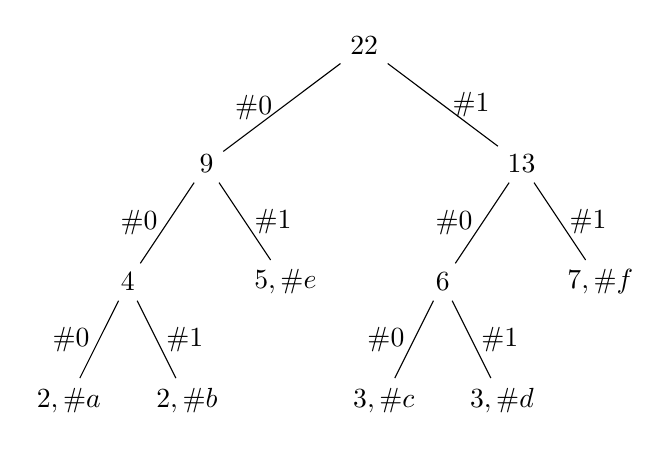
\begin{tikzpicture}
    [level 1/.style={sibling distance=40mm},
    level 2/.style={sibling distance=20mm},
    level 3/.style={sibling distance=15mm}]
    \node {$22$}
    child { node {$9$}
      child {node {$4$}
        child {node {$2, \#{a}$} 
          edge from parent node[left] {$\#0$}
        }
        child {node {$2, \#{b}$} 
          edge from parent node[right] {$\#1$}
        }
        edge from parent node[left] {$\#0$}
      }
      child {node {$5, \#{e}$} 
        edge from parent node[right] {$\#1$}
      }
      edge from parent node[left] {$\#0$}
    } 
    child { node {$13$}
      child { node {$6$}
        child {node {$3, \#{c}$}
          edge from parent node[left] {$\#0$}
        }
        child {node {$3, \#{d}$} 
          edge from parent node[right] {$\#1$}
        }
        edge from parent node[left] {$\#0$}
      }
      child { node {$7, \#{f}$} 
        edge from parent node[right] {$\#1$}
      }
      edge from parent node[right] {$\#1$}
    } ;
  \end{tikzpicture}
  \caption{Ein Beispielbaum für die Berechnung eines Huffman-Codes.}
  \label{abb:huffman-baum}
\end{figure}
% 
Wenn zum Beispiel das Wort $w=\#{afebfecaffdeddccefbeff}$ gegeben ist,
dann kann sich der Baum ergeben, der in
Abbildung~\ref{abb:huffman-baum} dargestellt ist.
%
In diesem Fall ist dann der Homomorphismus gegeben durch
\begin{center}
  \begin{tabular}{c@{\qquad}*{6}{>{$}c<{$}}}
    \toprule
    x & \#a & \#b& \#c& \#d& \#e& \#f \\
    h(x) & \#{000}& \#{001}& \#{100}& \#{101}& \#{01}& \#{11} \\
    \bottomrule
  \end{tabular}
\end{center}
%
Es bleibt zu beschreiben, wie man den Baum konstruiert.
% 
Zu jedem Zeitpunkt hat man eine Menge $M$ von "`noch zu betrachtenden
Symbolmengen mit ihren Häufigkeiten"'.
% 
Diese Menge ist initial die Menge aller $\{x\}$ für $x\in A$ mit den
zugehörigen Symbolhäufigkeiten, die wir so aufschreiben wollen:
\[
M_0= \{ \;(2,\{\#a\})\;, \;(2,\{\#b\})\;, \;(3,\{\#c\})\;,
\;(3,\{\#d\})\;, \;(5,\{\#e\})\;, \;(7,\{\#f\})\; \}
\]
Als Anfang für die Konstruktion des Baumes zeichnet man für jedes
Symbol einen Knoten mit Markierung $(x,N_x(w))$.
% 
Im Beispiel ergibt sich
\begin{center}
  \begin{tikzpicture}
    [level 1/.style={sibling distance=40mm},
    level 2/.style={sibling distance=20mm},
    level 3/.style={sibling distance=15mm}]
    \node {}%$22$}
    child { node {}%$9$}
      child {node {}%$4$}
        child {node {$2, \#{a}$} 
          edge from parent[draw=none]
        }
        child {node {$2, \#{b}$} 
          edge from parent[draw=none]
        }
        edge from parent[draw=none]
      }
      child {node {$5, \#{e}$} 
        edge from parent[draw=none]
      }
      edge from parent[draw=none]
    } 
    child { node {}%$13$}
      child { node {}%$6$}
        child {node {$3, \#{c}$}
          edge from parent[draw=none]
        }
        child {node {$3, \#{d}$} 
          edge from parent[draw=none]
        }
        edge from parent[draw=none]
      }
      child { node {$7, \#{f}$}
        edge from parent[draw=none]
      }
      edge from parent[draw=none]
    } ;
  \end{tikzpicture}
\end{center}

Solange eine Menge $M_i$ noch mindestens zwei Paare enthält, tut man folgendes:
\begin{itemize}
\item Man bestimmt man eine Menge $M_{i+1}$ wie folgt:
  \begin{itemize}
  \item Man wählt zwei Paare $(X_1,k_1)$ und $(X_2,k_2)$, deren
    Häufigkeiten zu den kleinsten noch vorkommenden gehören.
  \item Man entfernt diese Paare aus $M_i$ und fügt statt dessen das
    eine Paar $(X_1\cup X_2, k_1+k_2)$ hinzu. Das ergibt $M_{i+1}$.
  \end{itemize}
\end{itemize}
Im Beispiel ergibt sich also
\[
M_1= \{ \;(4,\{\#a,\#b\})\;, \;(3,\{\#c\})\;, \;(3,\{\#d\})\;, \;(5,\{\#e\})\;, \;(7,\{\#f\})\; \}
\]
\begin{itemize}
\item Als zweites fügt man dem schon konstruierten Teil des Graphen
  einen weiteren Knoten hinzu, markiert mit der Häufigkeit $k_1+k_2$
  und Kanten zu den Knoten, die für $(X_1,k_1)$ und $(X_2,k_2)$
  eingefügt worden waren
\end{itemize}

\begin{center}
  \begin{tikzpicture}
    [level 1/.style={sibling distance=40mm},
    level 2/.style={sibling distance=20mm},
    level 3/.style={sibling distance=15mm}]
    \node {}%$22$}
    child { node {}%$9$}
      child {node {$4$}
        child {node {$2, \#{a}$} 
        }
        child {node {$2, \#{b}$} 
        }
        edge from parent[draw=none]
      }
      child {node {$5, \#{e}$} 
        edge from parent[draw=none]
      }
      edge from parent[draw=none]
    } 
    child { node {}%$13$}
      child { node {}%$6$}
        child {node {$3, \#{c}$}
          edge from parent[draw=none]
        }
        child {node {$3, \#{d}$} 
          edge from parent[draw=none]
        }
        edge from parent[draw=none]
      }
      child { node {$7, \#{f}$}
        edge from parent[draw=none]
      }
      edge from parent[draw=none]
    } ;
  \end{tikzpicture}
\end{center}
%
Da $M_1$ noch mehr als ein Element enthält, wiederholt man die beiden
obigen Teilschritte:
\[
M_2= \{ \;(4,\{\#a,\#b\})\;, \;(6,\{\#c,\#d\})\;, \;(5,\{\#e\})\;, \;(7,\{\#f\})\; \}
\]
und der Graph sieht dann so aus:
%
\begin{center}
  \begin{tikzpicture}
    [level 1/.style={sibling distance=40mm},
    level 2/.style={sibling distance=20mm},
    level 3/.style={sibling distance=15mm}]
    \node {}%$22$}
    child { node {}%$9$}
      child {node {$4$}
        child {node {$2, \#{a}$} 
        }
        child {node {$2, \#{b}$} 
        }
        edge from parent[draw=none]
      }
      child {node {$5, \#{e}$} 
        edge from parent[draw=none]
      }
      edge from parent[draw=none]
    } 
    child { node {}%$13$}
      child { node {$6$}
        child {node {$3, \#{c}$}
        }
        child {node {$3, \#{d}$} 
        }
        edge from parent[draw=none]
      }
      child { node {$7, \#{f}$}
        edge from parent[draw=none]
      }
      edge from parent[draw=none]
    } ;
  \end{tikzpicture}
\end{center}
%
Da $M_2$ noch mehr als ein Element enthält, wiederholt man die beiden
obigen Teilschritte wieder:
\[
M_3= \{ \;(9,\{\#a,\#b,\#e\})\;, \;(6,\{\#c,\#d\})\;, \;(7,\{\#f\})\; \}
\]
und der Graph sieht dann so aus:
%
\begin{center}
  \begin{tikzpicture}
    [level 1/.style={sibling distance=40mm},
    level 2/.style={sibling distance=20mm},
    level 3/.style={sibling distance=15mm}]
    \node {}%$22$}
    child { node {$9$}
      child {node {$4$}
        child {node {$2, \#{a}$} 
        }
        child {node {$2, \#{b}$} 
        }
      }
      child {node {$5, \#{e}$} 
      }
      edge from parent[draw=none]
    } 
    child { node {}%$13$}
      child { node {$6$}
        child {node {$3, \#{c}$}
        }
        child {node {$3, \#{d}$} 
        }
        edge from parent[draw=none]
      }
      child { node {$7, \#{f}$}
        edge from parent[draw=none]
      }
      edge from parent[draw=none]
    } ;
  \end{tikzpicture}
\end{center}
%
Da $M_3$ noch mehr als ein Element enthält, wiederholt man die beiden
obigen Teilschritte wieder:
\[
M_4= \{ \;(9,\{\#a,\#b,\#e\})\;, \;(13,\{\#c,\#d,\#f\})\; \}
\]
und der Graph sieht dann so aus:
%
\begin{center}
  \begin{tikzpicture}
    [level 1/.style={sibling distance=40mm},
    level 2/.style={sibling distance=20mm},
    level 3/.style={sibling distance=15mm}]
    \node {}%$22$}
    child { node {$9$}
      child {node {$4$}
        child {node {$2, \#{a}$} 
        }
        child {node {$2, \#{b}$} 
        }
      }
      child {node {$5, \#{e}$} 
      }
      edge from parent[draw=none]
    } 
    child { node {$13$}
      child { node {$6$}
        child {node {$3, \#{c}$}
        }
        child {node {$3, \#{d}$} 
        }
      }
      child { node {$7, \#{f}$}
      }
      edge from parent[draw=none]
    } ;
  \end{tikzpicture}
\end{center}
%
Zum Schluss berechnet man noch
\[
M_5= \{ \;(22,\{\#a,\#b,\#c,\#d,\#e,\#f\})\; \}
\]
und es ergibt sich der Baum
\begin{center}
  \begin{tikzpicture}
    [level 1/.style={sibling distance=40mm},
    level 2/.style={sibling distance=20mm},
    level 3/.style={sibling distance=15mm}]
    \node {$22$}
    child { node {$9$}
      child {node {$4$}
        child {node {$2, \#{a}$} 
        }
        child {node {$2, \#{b}$} 
        }
      }
      child {node {$5, \#{e}$} 
      }
    } 
    child { node {$13$}
      child { node {$6$}
        child {node {$3, \#{c}$}
        }
        child {node {$3, \#{d}$} 
        }
      }
      child { node {$7, \#{f}$}
      }
    } ;
  \end{tikzpicture}
\end{center}
%
Aus diesem ergibt sich durch die Beschriftung der Kanten die
Darstellung in Abbildung~\ref{abb:huffman-baum}.

\begin{tutorium}
  Nehmen Sie acht Symbole: \#a, \#b, \#c, \#d, \#e, \#f, \#g, \#h
  \begin{itemize}
  \item 1. Fall: Jedes Zeichen kommt genau einmal vor.

    Huffman-Code-Baum erstellen, Wort \#{badcfehg} codieren, wie lang wird
    die Codierung?
    
  \item 2. Fall: \#a kommt einmal vor, \#b zweimal, \#c 4-mal, \#d 8-mal, \#e
    16-mal, \#f 32-mal, \#g 64-mal, \#h 128-mal.
    
    Huffman-Code-Baum erstellen, 

    Ergebnis \zB
    \begin{tabular}[t]{c@{\quad}*{8}{>{$}c<{$}}}
      \toprule
      x & \#a & \#b & \#c & \#d & \#e & \#f & \#g & \#h \\
      h(x) & \#{0000000}& \#{0000001}& \#{000001}& \#{00001}& \#{0001}& \#{001}& \#{01}& \#{1} \\
      \bottomrule
    \end{tabular}
 
    aber nicht das Wort $\#{abbcccc}\dots\#h^{128}$ codieren, sondern
    das Wort \#{badcfehg}; wie lang wird die Codierung?  \dots über
    $4$ mal so lang

  \item Wie lange wird ein Wort mit zweiter Zeichenverteilung, wenn
    man es mit dem ersten Code codiert? 

    Dreimal so lang, weil jeder
    Buchstabe durch $3$ Bits codiert wird.

  \item Wie lange wird ein Wort mit erster Zeichenverteilung, wenn man
    es mit dem zweiten Code codiert?

    

    Ziel: Sehen, dass Huffman-Codierung irgendwie zu funktionieren scheint.
  \end{itemize}
\end{tutorium}

% -----------------------------------------------------------------------
\Tut\subsection{Weiteres zu Huffman-Codes}

Wir haben das obige Beispiel so gewählt, dass immer eindeutig klar
war, welche zwei Knoten zu einem neuen zusammengefügt werden
mussten. 
% 
Im allgemeinen ist das nicht so: Betrachten Sie einfach den Fall, dass
viele Zeichen alle gleichhäufig vorkommen.
% 
Außerdem ist nicht festgelegt, welcher Knoten linker Nachfolger und
welcher rechter Nachfolger eines inneren Knotens wird.

Konsequenz dieser Mehrdeutigkeiten ist, dass ein Huffman-Code nicht
eindeutig ist. 
% 
Das macht aber nichts: alle, die sich für ein Wort $w$ ergeben können,
sind "`gleich gut"'.

Dass Huffman-Codes gut sind, kann man so präzisieren: unter allen
präfixfreien Codes führen Huffman-Codes zu kürzesten
Codierungen. 
% 
Einen Beweis findet man zum Beispiel unter
%\url{http://www.maths.abdn.ac.uk/~igc/tch/mx4002/notes/node59.html},  % geht nicht mehr
\url{http://web.archive.org/web/20090917093112/http://www.maths.abdn.ac.uk/~igc/tch/mx4002/notes/node59.html},
10.11.2015).

Zum Schluss wollen wir noch auf eine (von mehreren) Verallgemeinerung
des oben dargestellten Verfahrens hinweisen. 
% 
Manchmal ist es nützlich, nicht von den Häufigkeiten einzelner Symbole
auszugehen und für die Symbole einzeln Codes zu berechnen, sondern für
Teilwörter einer festen Länge $b>1$.
% 
Alles wird ganz analog durchgeführt; der einzige Unterschied besteht
darin, dass an den Blättern des Huffman-Baumes eben Wörter stehen und
nicht einzelne Symbole.

Eine solche Verallgemeinerung wird bei mehreren gängigen
Kompressionsverfahren (\zB gzip, bzip2) benutzt, die, zumindest als
einen Bestandteil, Huffman-Codierung benutzen.

Allgemein gesprochen handelt es sich bei diesem Vorgehen um eine
sogenannte \mdefine{Block-Codierung}\index{Block-Codierung}. 
% 
Statt wie bei einem Homomorphsimus die Übersetzung $h(x)$ jedes
einzelnen Zeichens $x\in A$ festzulegen, tut man das für alle
Teilwörter, die sogenannten Blöcke, einer bestimmten festen Länge
$b\in\N_+$.
% 
Man geht also von einer Funktion $h:A^b -> B^*$ aus, und erweitert
diese zu einer Funktion $h:(A^b)^* -> B^*$.

\begin{tutorium}
  \noindent\textbf{Blockcodierung mit Huffman}
  \begin{itemize}
  \item Verallgemeinerung: nicht von den Häufigkeiten einzelner
    Symbole ausgehen, sondern für Teilwörter einer festen Länge $b>1$
    die Häufigkeiten berechnen.
  \item Beispiel: Man hat einen Text über dem Alphabet $\{\#a, \#b,
    \#c, \#d\}$, der nur aus Teilwörtern der Länge $10$
    zusammengesetzt ist, die denen in jedem immer nur ein Symbol
    vorkommt, also \zB \#{aaaaaaaaaabbbbbbbbbbddddddddddcccccccccc}
    usw. Angenommen $\#a^{10}$, \dots, $\#d^{10}$ kommen alle gleich
    häufig vor. Wie lang ist dann die Huffman-Codierung?  Ein Fünftel,
    weil jeder Zehnerblock durch zwei Bits codiert wird.
  \end{itemize}
\end{tutorium}
% -----------------------------------------------------------------------
\section{Ausblick}

% Wir haben uns in dieser Einheit nur mit der Darstellung von
% nichtnegativen ganzen Zahlen beschäftigt. Wie man bei negativen und
% gebrochenen Zahlen \zB in einem Prozessor vorgeht, wird in einer
% Vorlesung über technische Informatik behandelt werden.

Wer Genaueres über UTF-8 und damit zusammenhängende Begriffe bei
Unicode wissen will, dem sei die detaillierte Darstellung im \emph{Unicode
  Technical Report UTR-17} empfohlen, den man unter
\url{http://www.unicode.org/reports/tr17/} (10.11.2015) im WWW findet.

Mehr über Bäume und andere Graphen werden wir in dem Kapitel mit dem
überraschenden Titel "`Graphen"' lernen.

\cleardoublepage

%-----------------------------------------------------------------------
%%%
%%% Local Variables:
%%% fill-column: 70
%%% mode: latex
%%% TeX-master: "../k-08-codierungen/skript.tex"
%%% TeX-command-default: "XPDFLaTeX"
%%% End:
